\section{Implementation quircks}

This section highlights a few of the most challenging non-functional aspects of this project. The explanations are related to the computational backend of the project that didn't find its place in the previous arcihtectural overview.

\subsection{The Neural Network inference architecture}

The two base classes Layer and Model provide the driver API for tensor teanformations. Each subclassed layer implements its own logic in the Call method, which for reasons of completitude feature a multi-input multi-output signature, despite the fact that at most two inputs are provided at one time (e.g. the Concatenate layer) and a single output tensor is always expected. Layer weights are provided by a LayerRuntimeContext class which simply wraps a dictionary of keys and tensors. This resulted as a decision to clearly separate layer definition/architecture from its numerical state. Each Layer class contains a list of references input layer referenced. By choosing the output layer and consequently following the input layers, we can trace a tree structure roughly equivalent to an execution graph with reverse orientation. This fact is used by the Model class in a rudimentary queue-based algorithm to decide the order of processing layers. This approach works well for the scope of the problem since an almost sequential flow is guaranteed therefore linear complexity of the graph traversal is assured.

\begin{figure}[htbp]
	\centering
		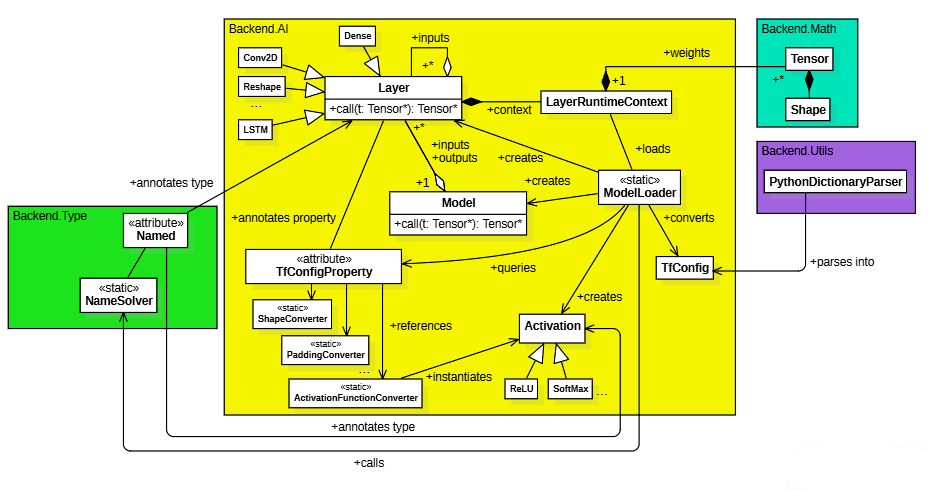
\includegraphics[scale=0.6]{figures/diagram_backend_ai.png}
	\caption{Backend AI ecosystem}
        \label{FigDiagramAI}
\end{figure}

\subsection{Porting the neural network into native language}
\label{subsec:ch6sec4subsec1}

A significant effort has been put into making the model arhitectures and especially the trained weights accessible in C\# with as little developer intervention as possible while preserving loading time performance. The model deployment pipeline consists of two steps. First, a Python script loads the model saved in a traditional format (e.g. HDF5 or Tensorflow custom own format) and outputs essential information about each layer like its name, type, inputs, shapes. The weights are encoded as sequences of floating point hexadecimal number to prevent unwanted precision errors. The most important element to keep track of is the layer configuration (obtained by calling Tensorflow Layer.get\_config() method), as it contains valuable information about layer function and hyperparameters. This first step was needed for debugging purposes and can definitely be skipped, albeit it increases comprehension by focusing solely on the data that needs encoded. In the next step, another executable rearranges the data obtained so far into a binary format, which as expected boosts the reading time by eliminating parsing redundancies in a loader code. This process involves a minutiose work on the developer side. On the backend, each layer class has been annotated with a Named attribute which makes it automatically visible to a NameSolver mechanism that creates a new instance of a Named type by reflection. The same type naming system is used for activation functions to allow instantiating the correct class from a key-value pair like "activation:'softmax'". Furthermore, another annotation TfConfigProperty placed on Layer-derived class properties facilitates the inference of configuration properties directly from a dictionary data loaded from a binary file. An optional converter class plays the role of a deserializer in case a layer needs a piece of data to be treated in a particular way (e.g. an array originating from a Python tuple that describes a tensor Shape object). Finally, the entire file loading and model construction process is being taken care of a static ModelLoader class. With the help of the C\# assembly resources manager, instantiating a model becomes as simple as "var model = ModelLoader.LoadFromBytes(Resources.MyEncodedModelBytes)". This system is easily scalable, since adding a new layer type only requires declaring the Named attribute of the class, specifying the config properties and the tensor operations logic.

\subsection{Deserialization of Python dictionaries}
\label{subsec:ch6sec4subsec2}

An unfortunate choice of design had led to passing the layer configuration as a native Python dictionary string to the C\# backend at layer porting time instead of translating it into an easier to diggest structure using the Python script. This incident crystallized into an off-topic mission to write a custom Pyton to C\# object converter. A series of finite automata is used to extract lexical atoms from the dictionary string, which are passed to a LR-1 analyzer which also translates data on the fly to internal object representation. The process will not be detailed here, since it is outside the scope of the thesis, however, it is worth mentioning its instructive value as a formal languages practical exercise.  